\documentclass[a4paper,listof=leveldown,listof=numbered]{scrreprt}

\usepackage[ngerman]{babel}
\usepackage[utf8]{inputenc}
\usepackage[T1]{fontenc}
\usepackage{todonotes}
\usepackage{ae}
\usepackage{float}
\usepackage{booktabs}
\usepackage{multirow}
\usepackage{colortbl}
\usepackage{tabularx}
\usepackage[printonlyused]{acronym}
\usepackage[automark,headsepline,ilines,komastyle, plainfootsepline]{scrpage2} 
\usepackage[bookmarks,bookmarksnumbered]{hyperref}

\newcommand{\gray}{\rowcolor[gray]{.90}}

%Kopf- und Fußzeile---------------------------
\pagestyle{scrheadings}
\clearscrheadings
\lohead{\headmark}
\rohead{Software-Engineering Gruppenarbeit}
\lofoot[Gmeiner, Rezmer, Zeiler]{Gmeiner, Rezmer, Zeiler}
\cofoot{\pagemark}
\rofoot[\today]{\today}
\cfoot{\pagemark}
\setheadsepline{.4pt} % Linie unter dem Head
\setfootsepline{.4pt} % Ganzunten
%---------------------------------------------

\begin{document}
	\begin{titlepage}

\begin{center}


% Oberer Teil der Titelseite: Firmenlogo/Projektlogo
%\includegraphics[width=0.15\textwidth]{./logo}\\[1cm]    

\textsc{\LARGE TINF13IN GmbH}\\[2cm]

\textsc{\Large Pflichtenheft für}\\[1 cm]


% Title
\newcommand{\HRule}{\rule{\linewidth}{0.5mm}}
\HRule \\[0.4cm]
{\fontsize{60}{65} \bfseries \selectfont ScOREO}\\ [0.4cm]

\HRule \\[2.5cm]

% Author and supervisor
\begin{minipage}{0.4\textwidth}
\begin{flushleft} 
\end{flushleft}
\end{minipage}
\hfill
\begin{minipage}{0.4\textwidth}
\begin{flushright} \large
\emph{erstellt von:} \\
Alexander \textsc{Rezmer}\\
Fabian \textsc{Zeiler}\\
Christian \textsc{Gmeiner}
\end{flushright}
\end{minipage}

\vfill

% Unterer Teil der Seite
\large
{\large \today\\
\emph{Version:} v0.9}

\end{center}

\end{titlepage}
	
	% Platzierung des Inhaltsverzeichnisses
	\tableofcontents
	
\chapter{Zielbestimmung}
	Das im Folgenden beschriebene Programm soll die Grundlage für ein Bewertungssystem für Prüfer sein. Mit diesem System soll eine gerechte und einfache Bewertung ermöglicht werden. Dies wird sichergestellt indem die einzelnen Bewertungen auf einen gemeinsamen Score umgerechnet werden. Durch verschiedene Gewichtungen der Scores ergibt sich die Möglichkeit einzelne Bewertungen stärker zu werten als andere. Eine weitere Funktionalität des Programmes soll es dem Prüfer ermöglichen zum Score ebenfalls eine Rückmeldung anzuhängen um dem Prüfling ein Feedback zu geben. Genau so soll der Prüfling (ggf. Student) ein Feedback anfordern können um eine Begründung zu für seine Bewertung erhalten zu können.
	
	\section{Musskriterien}
	Die Software muss eine korrekte Umrechnung der Bewertungen in gültige Scores beherrschen, welche die Prüfer eintragen. Da es sich bei diesen um teilweise sensible Daten handelt, müssen diese gut geschützt sein, sodass sie von außerhalb nicht verändert werden können. Dieses Programm bietet die Möglichkeit durch ein zweistufiges holistisches Bewertungssystem die Bewertungen einzutragen. Bei diesem zweistufigen System kann der Prüfer die Stufen selbst so gewichten wie er es für sinnvoll hält. Mehrere Bewertungen können miteinander verrechnet und einzeln gewichtet werden. Am Ende soll der Prüfer ein Score bekommen, welcher sich aus seinen Bewertungen und Gewichtungen errechnen lässt. Die Software muss auf Windows PCs lauffähig sein, da dies die am meisten verwendete Laufzeitumgebung ist. Des weiteren muss das System einfach zu bedienen sein. Der Prüfer muss die Ergebnis seiner Bewertung einfach an die Studenten weiter geben können. Dies kann durch einen Ausdruck dieser statt finden wie auch durch ein eigenes Programm welches den Studenten Zugriff auf die jeweiligen Scores liefert. Umrechnung von der Inversen muss auch voll funktionsfähig sein. 
	
	\section{Wunschkriterien}
	Das Grundprogramm soll wie ein Gerüst dienen, sodass man verschiedene \acs{Add-On} einbinden kann. Dieses Zusatzapplikationen können weitere Bewertungsmöglichkeiten beziehungsweise Umrechnungen zwischen diesen Bewertungen sein. Es kann sich dabei auch um eine Anbindung an bestehende Systeme verschiedener anderer Anbieter handeln. Später, wenn das Backend funktionsfähig ist, soll durch eine Website ein Zugriff ermöglicht werden um von Mobilen Endgeräte oder jedem anderen Gerät welches einen Browser besitzt darauf zugreifen zu können. Des weiteren soll eine \ac{API} implementiert werden, mit welcher andere Programme mit diesem Programm kommunizieren können. Es soll eine iOS App erstellt werden um bequem von iPad/iPhone darauf zugreifen zu können.
	
	\section{Abgrenzungskriterien}
	Das Produkt soll keine Software werden, mit welcher die Studenten untereinander verglichen werden. Dies kann gegebenen falls durch \acs{Add-On} ermöglicht werden, es gehört jedoch nicht zu diesem Projekt dazu. Des weiteren soll die Software kein Netzwerk darbieten in welchem unterschiedlichen Prüfer sich mit anderen austauschen können und die Prüfungsergebnisse untereinander vergleichen zu können.
	
\chapter{Produkteinsatz}
	Der geplante Einsatz des Systems ist die Grundlage für Benutzungsoberfläche und Qualitätsanforderungen.
	
	\section{Anwendungsbereiche}
	Das System soll vor allem zur Bewertung von Schülern und Studenten dienen. Es können jedoch auch andere Institutionen oder Firmen, welche ein einheitliches Bewertungssystem wollen, welches eine faire Bewertung ermöglicht. Es muss jedoch garantiert werden, dass keine fremden Personen Zugriff auf das System bekommen, da es sich bei solchen Bewertungen um teils sensible Informationen handelt. Studenten sollten die einfache Möglichkeit besitzen nachdem sie einen Test durchlaufen haben ihre Bewertung zu erfahren und diese auf einer einfachen Oberfläche teils grafisch dargestellt werden soll um einen Vergleich zu ermöglichen.
	
	\section{Zielgruppen}
	\begin{itemize}
		\item \underline{Prüfer:}\\
	Der Prüfer ist der Ersteller sowie der Bearbeiter der Prüfung. Dieser muss sich sinnvolle Bewertungskriterien überlegen, sowie in das System eintragen. Der Prüfer benötigt alle Funktionen zum Eintragen der Bewertungen bzw. der Scores.
	
		\item \underline{Hochschulen:}\\
	Das System soll transparent für verschiedene Hochschulen verwendet werden.  Die Bewertungskriterien sind einfach anpassbar an die jeweiligen Hochschulverordnungen. Zusätzlich sind individuelle Bewertungskriterien stets möglich.
			
		\item \underline{Sekretärin:}\\
	Die Sekretärin Benötigt zugriff auf das System um die Score auslesen zu können. Die Scores werden in einem Archiv abgespeichert und für 10 Jahre hinterlegt. 	
		
	\end{itemize}

	\section{Betriebsbedingungen}
	\begin{itemize}
	\item \underline{Physikalische Umgebung: Mobiler Laptop Einsatz} \\
	Der Prüfer sollte den Client immer Verfügbar haben. Dieser sollte mobil auf einem Laptop funktionieren. Die Datenbank abfragen befinden sich auf einem Server. Später sollte es möglich sein, per Webbrowser auf die Anwendung zuzugreifen.
	
	\item \underline{Tägliche Betriebszeit: dauerhaft} \\
	Der Server sollte dauerhaft verfügbar sein, damit der Prüfer ständig auf die Anwendung zugreifen kann. 
	
	\item \underline{Betrieb: Unbeaufsichtigter Betrieb} \\
	Sobald der Server einmal installiert ist, sollte das System ohne weitere Konfigurationen funktionieren. Der Prüfer sollte sich nicht mit der Konfiguration des System belasten müssten. 
	
	\end{itemize}
	
\chapter{Produktübersicht}
	\begin{figure}[H]
		\centering
		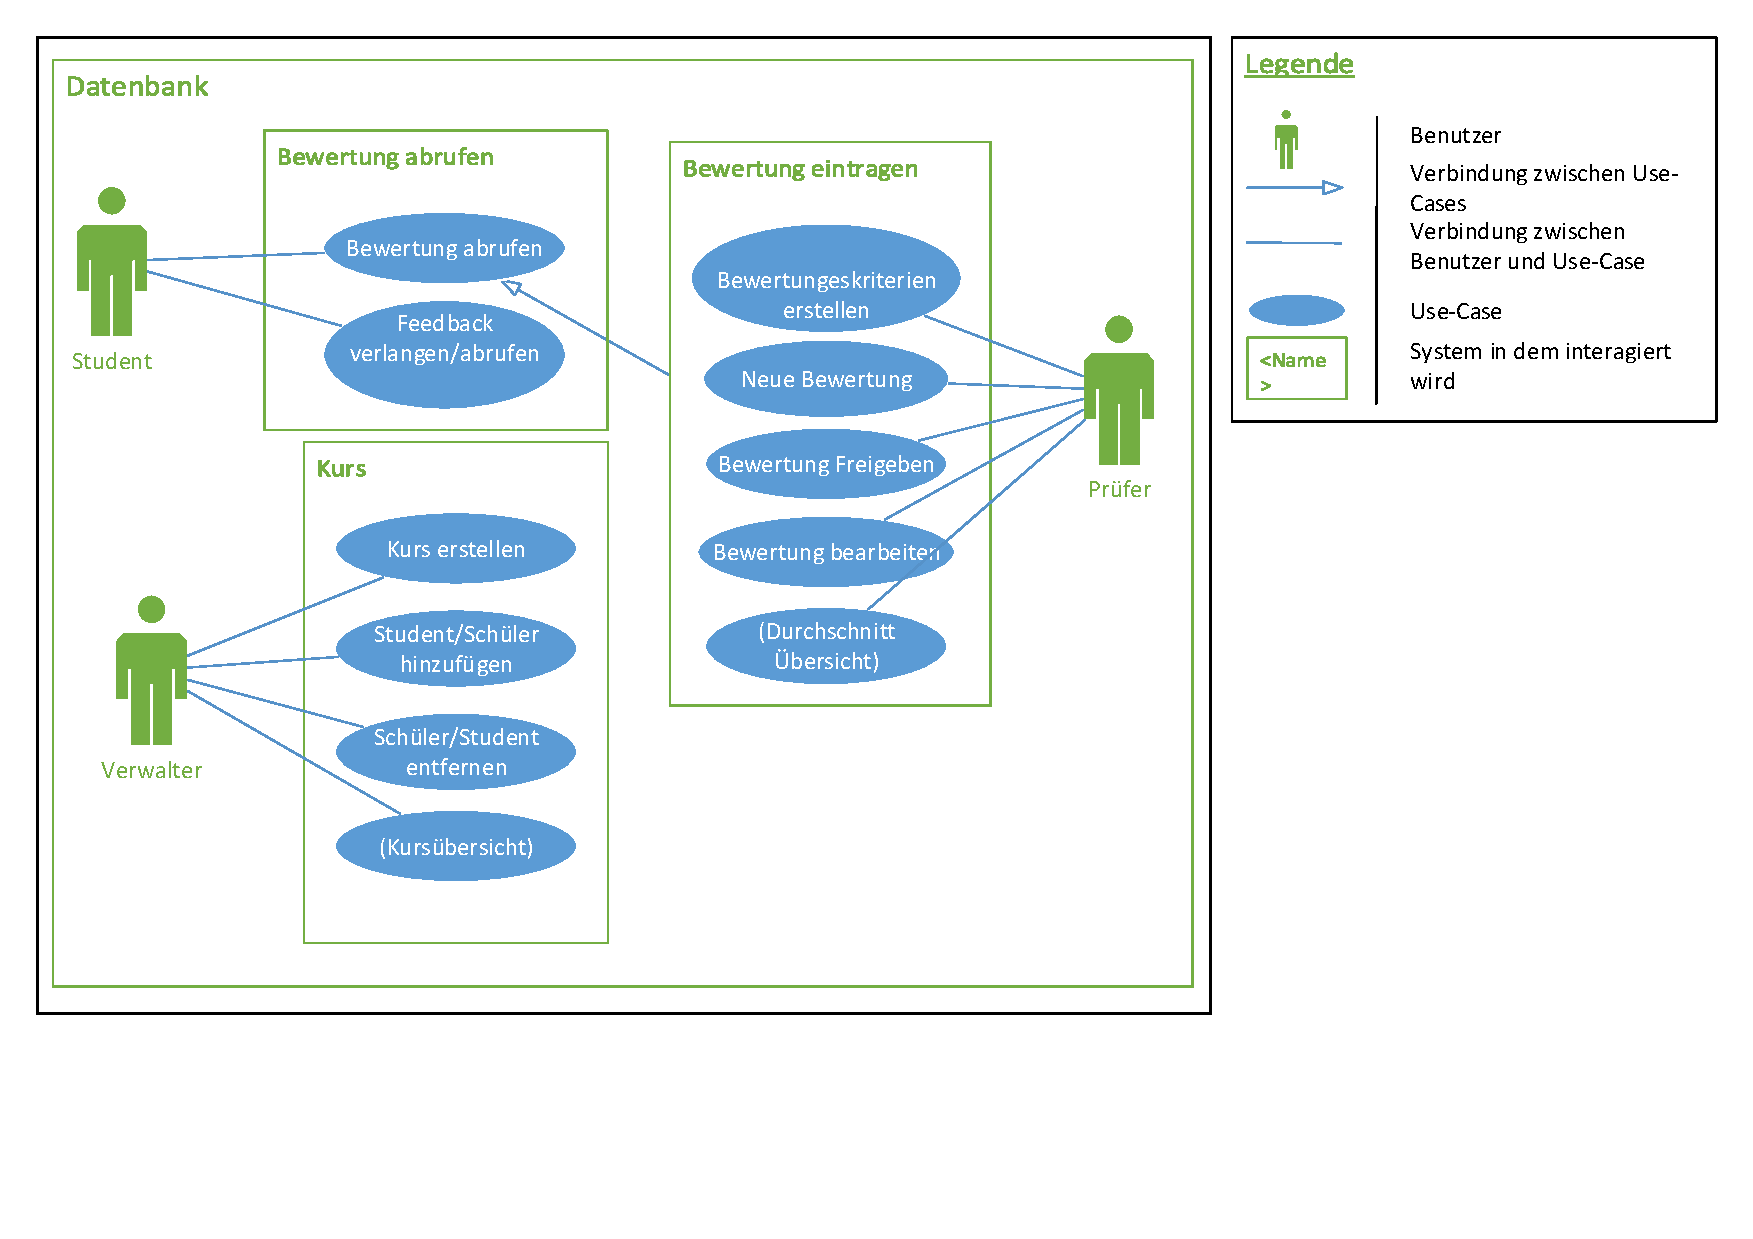
\includegraphics[width=0.99\textwidth]{../Use_Case.pdf}
		\caption{Use-Case Szenario}
	\end{figure}

	
\chapter{Produktfunktionen}
	\begin{figure}[H]
		\centering
		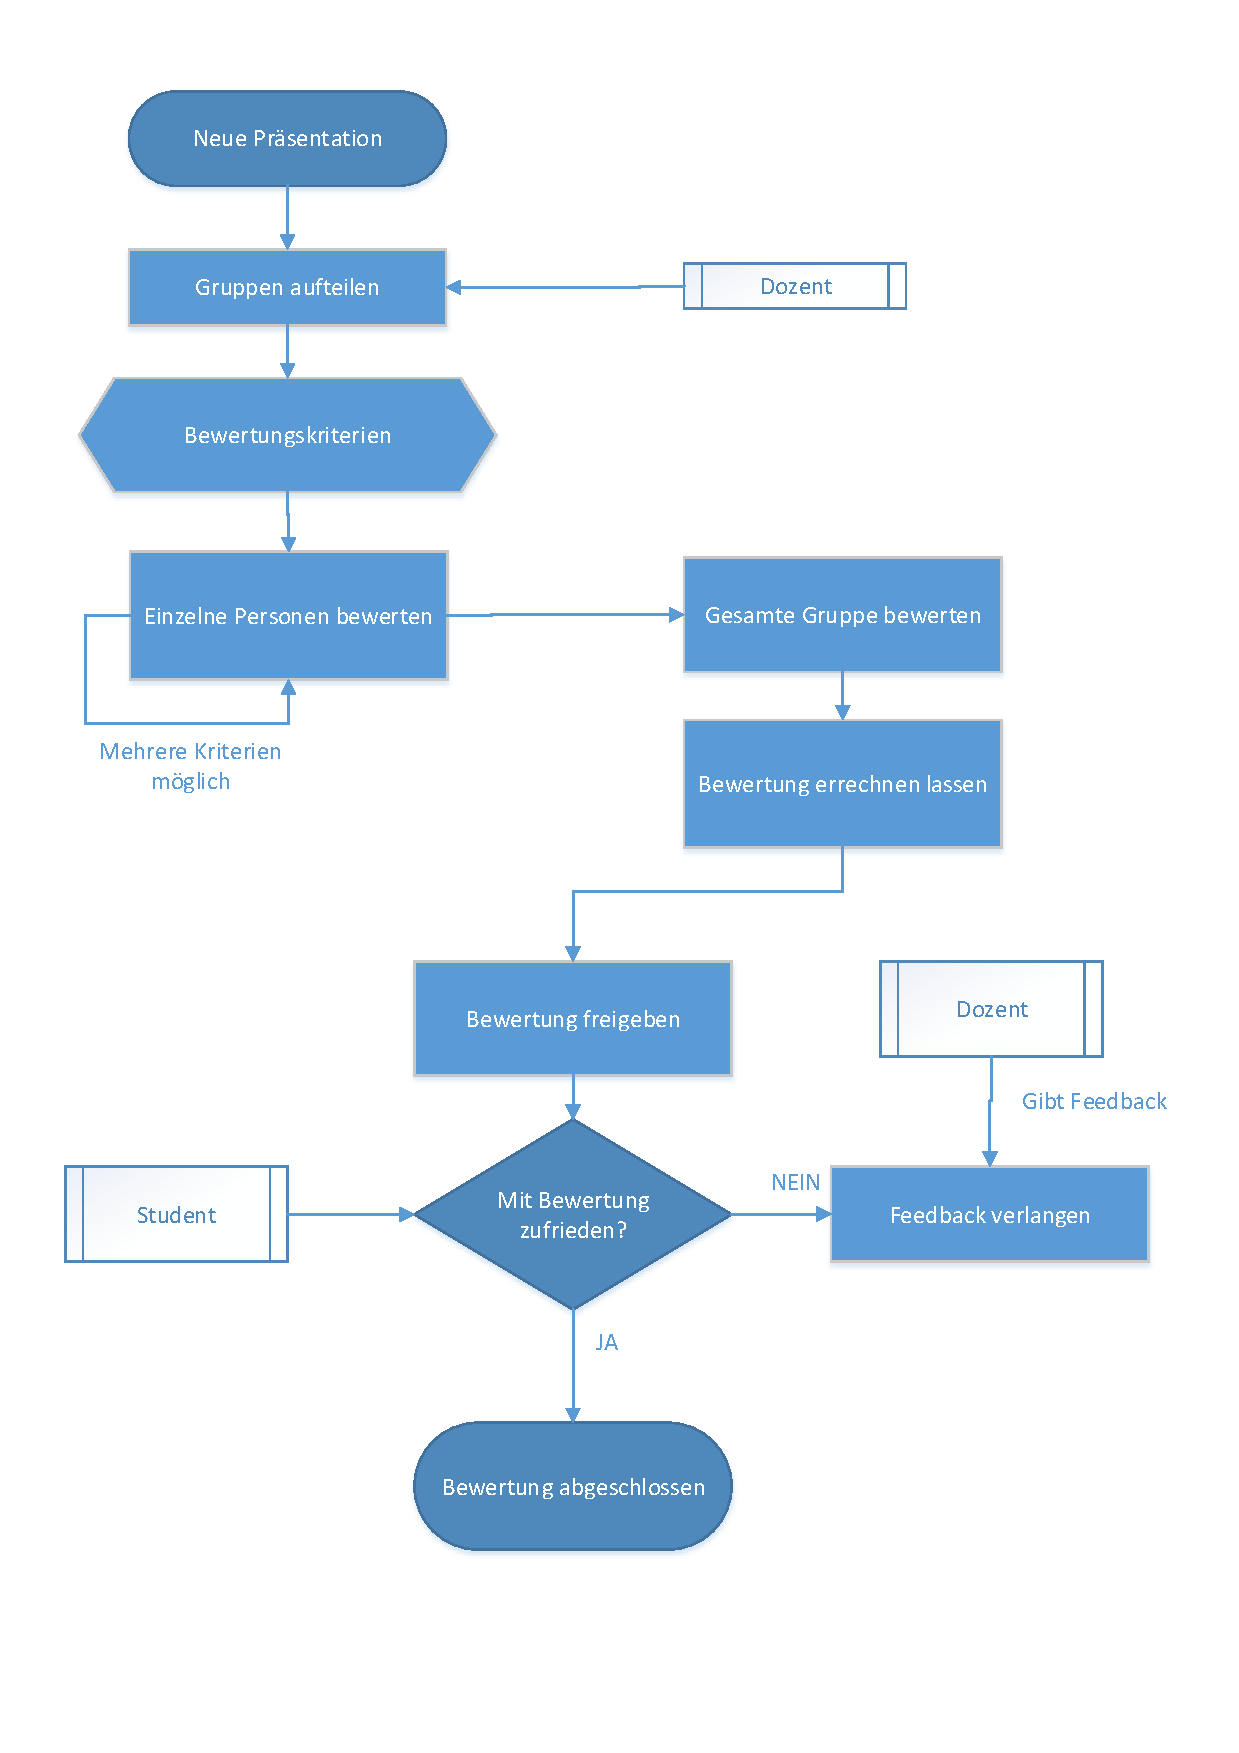
\includegraphics[height=0.8\textheight]{../Beispielprozess.pdf}
		\caption{Beispielprozess einer Bewertung}
	\end{figure}
	
\chapter{Produktdaten}
	In den Produktdaten sollten enthalten sein:
	\begin{itemize}
		\item Name des Studenten
		\item Vorname des Studenten
		\item Matrikelnummer des Studenten
		\item Die "`Endscores"' des Studenten
		\item "`Zwischenscores"' 
		\item Fach vom Score 
	\end{itemize}
	Insgesamt können von jedem Studenten mehrere Score eingetragen werden. Name, Vorname und Matrikelnummer sind nur einmal in der Datenbank hinterlegt um Redundanz zu verhindern. 
	

\chapter{Produktleistungen}
	Die Software soll eine Stabilität enthalten, wodurch mehrere Studenten/Dozenten auf einmal darauf zugreifen können.
	
\chapter{Qualitätsanforderungen}
	\chapter{Qualitätsanforderungen}

%Qualitätsanforderungen	
\begin{table}[H]
	\centering
	\caption{Qualitätsanforderungen}
	\begin{tabularx}{\textwidth}{l|X|X|X|X}
		\toprule
		\textbf{Produktqualität}       & \centering \textbf{sehr gu}t & \centering \textbf{gut}      & \centering \textbf{normal}   & \textbf{irrelevant} \\
		\toprule
		\multicolumn{5}{l}{\textbf{Funktionalität}}                           \\ 
		\midrule
		\quad Angemessenheit        &          &          & $\times$ &  \\ \hline
		\quad Richtigkeit           &          &  $\times$ &          &  \\ \hline
		\quad Interoperabilität     &          &          & $\times$ &  \\ \hline
		\quad Ordnungsmäßigkeit     &          & $\times$ &          &  \\ \hline
		\quad Sicherheit            &          & $\times$ &          &  \\
		\toprule
		\multicolumn{5}{l}{\textbf{Zuverlässigkeit}}                          \\
		\midrule
		\quad Reife                 &          & $\times$ &          &  \\ \hline
		\quad Fehlertolleranz       &          &          & $\times$ &  \\ \hline
		\quad Wiederherstellbarkeit &          &          & $\times$ &  \\ 
		\toprule
		\multicolumn{5}{l}{\textbf{Benutzbarkeit}}                            \\ 
		\midrule
		\quad Verständlichkeit      & $\times$ &          &          &  \\ \hline
		\quad Erlernbarkeit         & $\times$ &          &          &  \\ \hline
		\quad Bedienbarkeit         & $\times$ &          &          &  \\ 
		\toprule
		\multicolumn{5}{l}{\textbf{Effizienz}}                                \\
		\midrule
		\quad Zeitverhalten         &          &          &          & $\times$       \\ \hline
		\quad Verbrauchsverhalten   &          &          & $\times$ &  \\ 
		\toprule
		\multicolumn{5}{l}{\textbf{Änderbarkeit}}                             \\ 
		\midrule
		\quad Analysierbarkeit      &          &          & $\times$ &  \\ \hline
		\quad Modifizierbarkeit     &          &          &          & $\times$       \\ \hline
		\quad Stabilität            &          &          & \centering  $\times$ &  \\ \hline
		\quad Prüfbarkeit           &          &          & \centering $\times$ &  \\ 
		\toprule
		\multicolumn{5}{l}{\textbf{Übertragbarkeit}}                          \\ 
		\midrule
		\quad Anpassbarkeit         &          &          &          & $\times$       \\ \hline
		\quad Installierbarkeit     &          &          &          & $\times$       \\ \hline
		\quad Konformität           &          &          & $\times$ &  \\ \hline
		\quad Austauschbarkeit      &          &          &          & $\times$       \\ \hline
	\end{tabularx}%
	\label{tab:QualAnfor}%
\end{table}%
	
	\begin{itemize}
		\item Funktionalität:\\
		In der Rubrik Funktionalität spielt vor allem die Sicherheit eine große Rolle, weshalb die Qualitätsanforderungen hier sehr gut sein müssen. Es muss garantiert werden, dass keine Daten geklaut oder missbraucht werden können. Deshalb ist es ratsam hier mehr Zeit zu investieren. Die Punkte Richtigkeit und Ordnungsmäßigkeit müssen qualitativ nicht so hochwertig sein wie die Sicherheit, weil kleine Pannen bei der Benutzung keine gravierenden Schäden anrichten. Normale Qualität genügt bei Angemessenheit und Interoperabilität.\\
		
		\item Zuverlässigkeit:\\
		Insgesamt sollte das Programm zuverlässig laufen, jedoch müssen nicht überwiegend Ressourcen dafür verbraucht werden. Sollte das System abstürzen oder nicht ordnungsgemäß laufen, kann man nach einem Neustart weiterarbeiten.\\
		
		\item Benutzbarkeit:\\
		Viel Augenmerk wird auf die Benutzbarkeit gelegt. Das Programm sollte für den Anwender einfach zu bedienen sein und sich selbst erklären, damit keine Schulung mehr notwendig ist. \\
		
		\item 	Effizienz:\\
		Ausschlaggebend ist die Effizienz nicht, da das Bewertungssystem nicht besonders schnell die Score abrufen und verarbeiten muss. \\
		
		\item Änderbarkeit:		
		Für die Zukunft können weitere Features eingebaut werden, wenn man möchte. Grundsteine für weitere Features werden nicht gezielt gelegt.\\
					
		\item  Übertragbarkeit:
		Die Übertragbarkeit spielt eine untergeordnete Rolle, da man nur drauf zugreifen muss. Installieren oder ähnliches muss nicht getan werden. \\
			
	\end{itemize}
	
	
	
	\begin{itemize}
		\item Funktionalität:\\
		In der Rubrik Funktionalität spielt vor allem die Sicherheit eine große Rolle, weshalb die Qualitätsanforderungen hier sehr gut sein müssen. Es muss garantiert werden, dass keine Daten geklaut oder missbraucht werden können. Deshalb ist es ratsam hier mehr Zeit zu investieren. Die Punkte Richtigkeit und Ordnungsmäßigkeit müssen qualitativ nicht so hochwertig sein wie die Sicherheit, weil kleine Pannen bei der Benutzung keine gravierenden Schäden anrichten. Normale Qualität genügt bei Angemessenheit und Interoperabilität.\\
		
		\item Zuverlässigkeit:\\
		Insgesamt sollte das Programm zuverlässig laufen, jedoch müssen nicht überwiegend Ressourcen dafür verbraucht werden. Sollte das System abstürzen oder nicht ordnungsgemäß laufen, kann man nach einem Neustart weiterarbeiten.\\
		
		\item Benutzbarkeit:\\
		Viel Augenmerk wird auf die Benutzbarkeit gelegt. Das Programm sollte für den Anwender einfach zu bedienen sein und sich selbst erklären, damit keine Schulung mehr notwendig ist. \\
		
		\item 	Effizienz:\\
		Ausschlaggebend ist die Effizienz nicht, da das Bewertungssystem nicht besonders schnell die Score abrufen und verarbeiten muss. \\
		
		\item Änderbarkeit:
		
		Für die Zukunft können weitere Features eingebaut werden, wenn man möchte. Grundsteine für weitere Features werden nicht gezielt gelegt.\\
		
			
		\item  Übertragbarkeit:
		
		Die Übertragbarkeit spielt eine untergeordnete Rolle, da man nur drauf zugreifen muss. Installieren oder ähnliches muss nicht getan werden. \\
			
	\end{itemize}
	
\chapter{Benutzungsoberfläche}
	\begin{itemize}
		\item Intuitive Bedienung
		\item Selbsterklärend
		\item Ansprechendes Design
	\end{itemize}
	
\chapter{Technische Produktumgebung}
	Auf dem Server wird eine CoucDB-Datenbank verwendet. Auf der Clientseite wird ein Java – Programm installiert. Da wir in der Vergangenheit sehr gute Ergebnisse mit Java und einer CouchDB-Datenbank erzielt haben werden wir dies auch bei diesem Projekt verwenden.
	
	\section{Software}
	\begin{itemize}
		\item Betriebssystem : Windows 7, Windows 8, Windows 8.1
		\item Laufzeitsystem: JRE
		\item Datenbank: CouchDB
		\item Client: Java Programm
	\end{itemize}

	\section{Hardware}
	\begin{itemize}
		\item Mindestanforderungen für CouchDB: 32-Bit Betriebssystem
		\item Mindestanforderungen für Client: JRE, Windows 7
	\end{itemize}

	\section{Orgware}
	Internet Zugang
	
	\section{Produkt-Schnittstellen}
	Anbindung von Java und CoucDB über JSON.
	
\chapter{Spezielle Anforderungen an die Entwicklungs-Umgebung}
	
	\section{Software}
	Als Software für die Entwicklung wird Windows 7 und Mac OSX 10.10 verwendet, da diese Systeme zur Verfügung stehen. Des weiteren wird Eclipse als IDE für Java verwendet. Um die Daten abzulegen wird eine CouchDB Datenbank verwendet.
	\section{Hardware}
	Windows 7\\
	
	MacBook Pro 13"
	\begin{itemize}
		\item OS: Mac OSX 10.10
		\item Intel Core2Duo
	\end{itemize}
	Mac OSX 10.10
	
	\section{Orgware}
	Internet Zugang
	
	\section{Produkt-Schnittstellen}
	Internetanbindung von Java und CouchDB Datenbank.

	
\chapter{Gliederung in Teilprodukte}
	Drei Teilprodukte
	\begin{itemize}
		\item Logik 
			\begin{itemize}
				\item Zweistufige holistische Bewertung (H2)
				\item Rate-to-Score (R2S)
				\item Score-to-Rate (S2R)
			\end{itemize}
		\item GUI
		\item Backend (Datenbankanbindung inkl. Benutzerauthentifizierung)
	\end{itemize}

%\chapter{Ergänzungen}	
%	In diesem Kapitel werden Ergänzungen sowie spezielle Anforderungen beschrieben die über die aufgeführten Kapitel 1 bis 12 hinausgehen. Beispielsweise können hier Installationsbedingungen festgelegt werden wie:\\
%	bauliche und räumliche Voraussetzungen\\
%	Bereitstellung von Testdaten\\
%	Bereitstellung von Hilfspersonal\\
%	Außerdem können hier zu berücksichtigende\\
%	Normen\\
%	Vorschriften\\
%	Patente und\\
%	Lizenzen aufgeführt werden.
	
\chapter{Anhang}
\appendix
	\section{Begriffsdefinitionen}

	\section{Abkürzungsverzeichnis}
		\begin{acronym} 
			% Acronym mit \acro hinzu
			\acro{API}{Application Programming Interface (Programmierschnittstelle)}
			\acro{Add-On}{Erweiterungspaket}
		\end{acronym}
	
	% Abbildungsverzeichnis
	\listoffigures
	
	\section{Aufwandsabschätzung}
	%Aufwandsabschätzungstabelle einfügen
	\begin{figure}
		\centering
		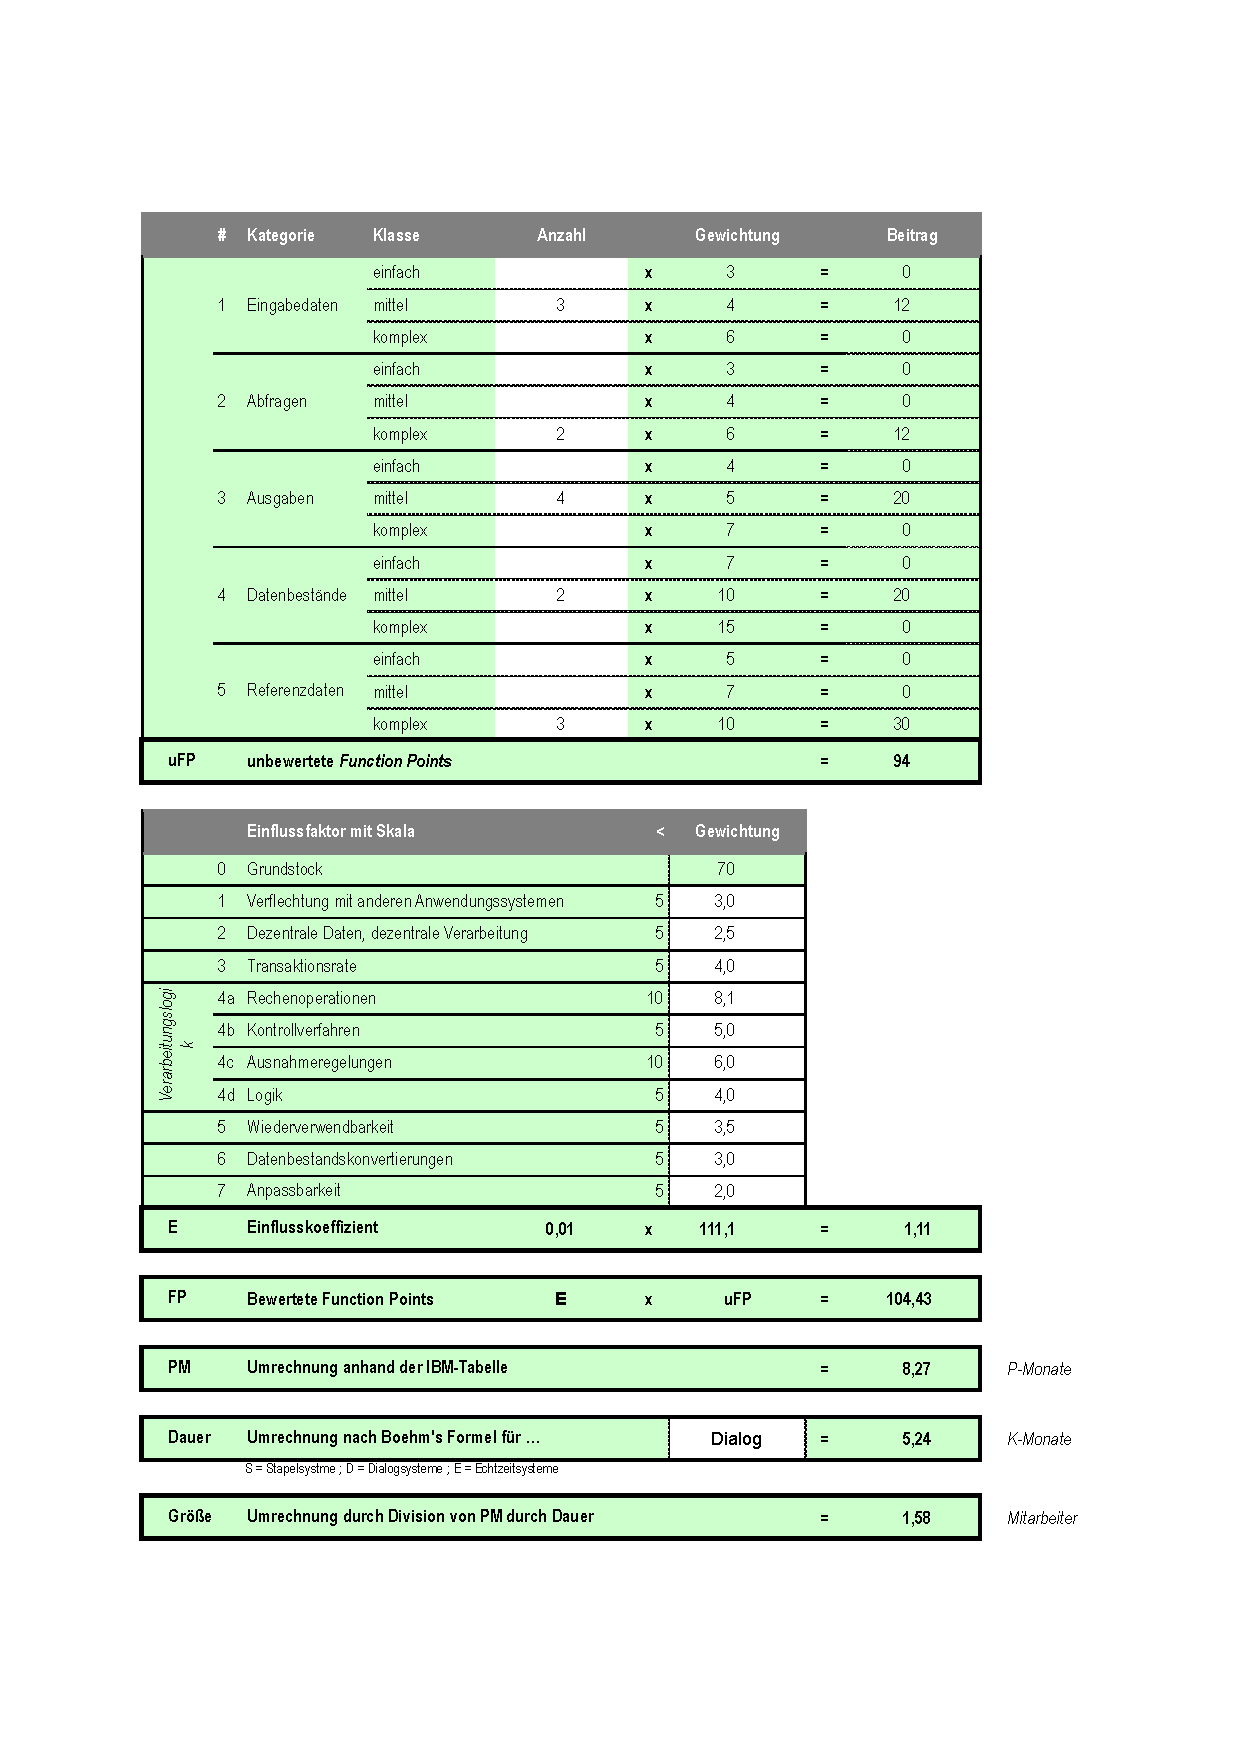
\includegraphics[width=0.99\textwidth]{data/Aufwandsabschaetzung.pdf}
	\end{figure}
	
	\section{Datenflussdiagramme}
	\begin{figure}
		\centering
		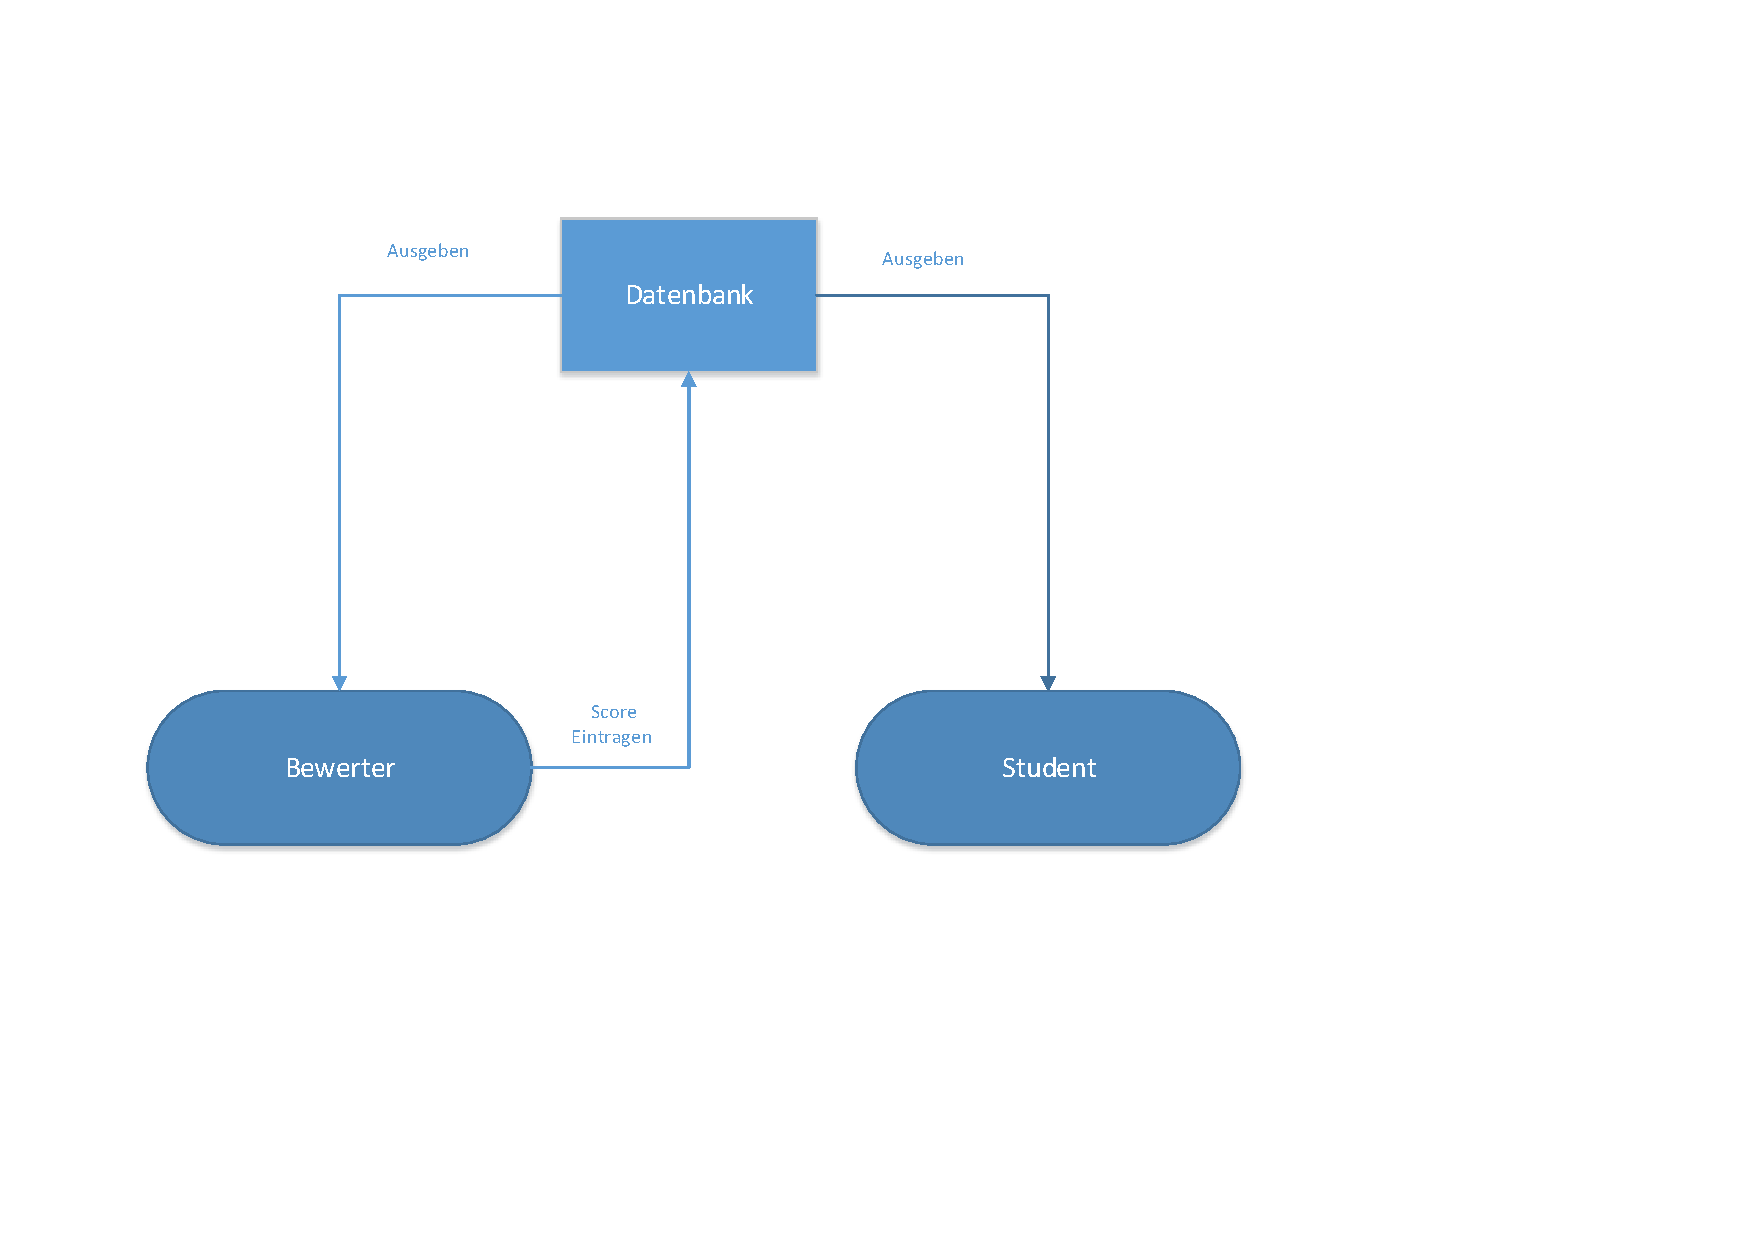
\includegraphics[width=0.7\textwidth]{img/DTD_1_BewerterStudent.pdf}
		\caption{Datenfluss Bewerter-Student}
	\end{figure}
	\begin{figure}
		\centering
		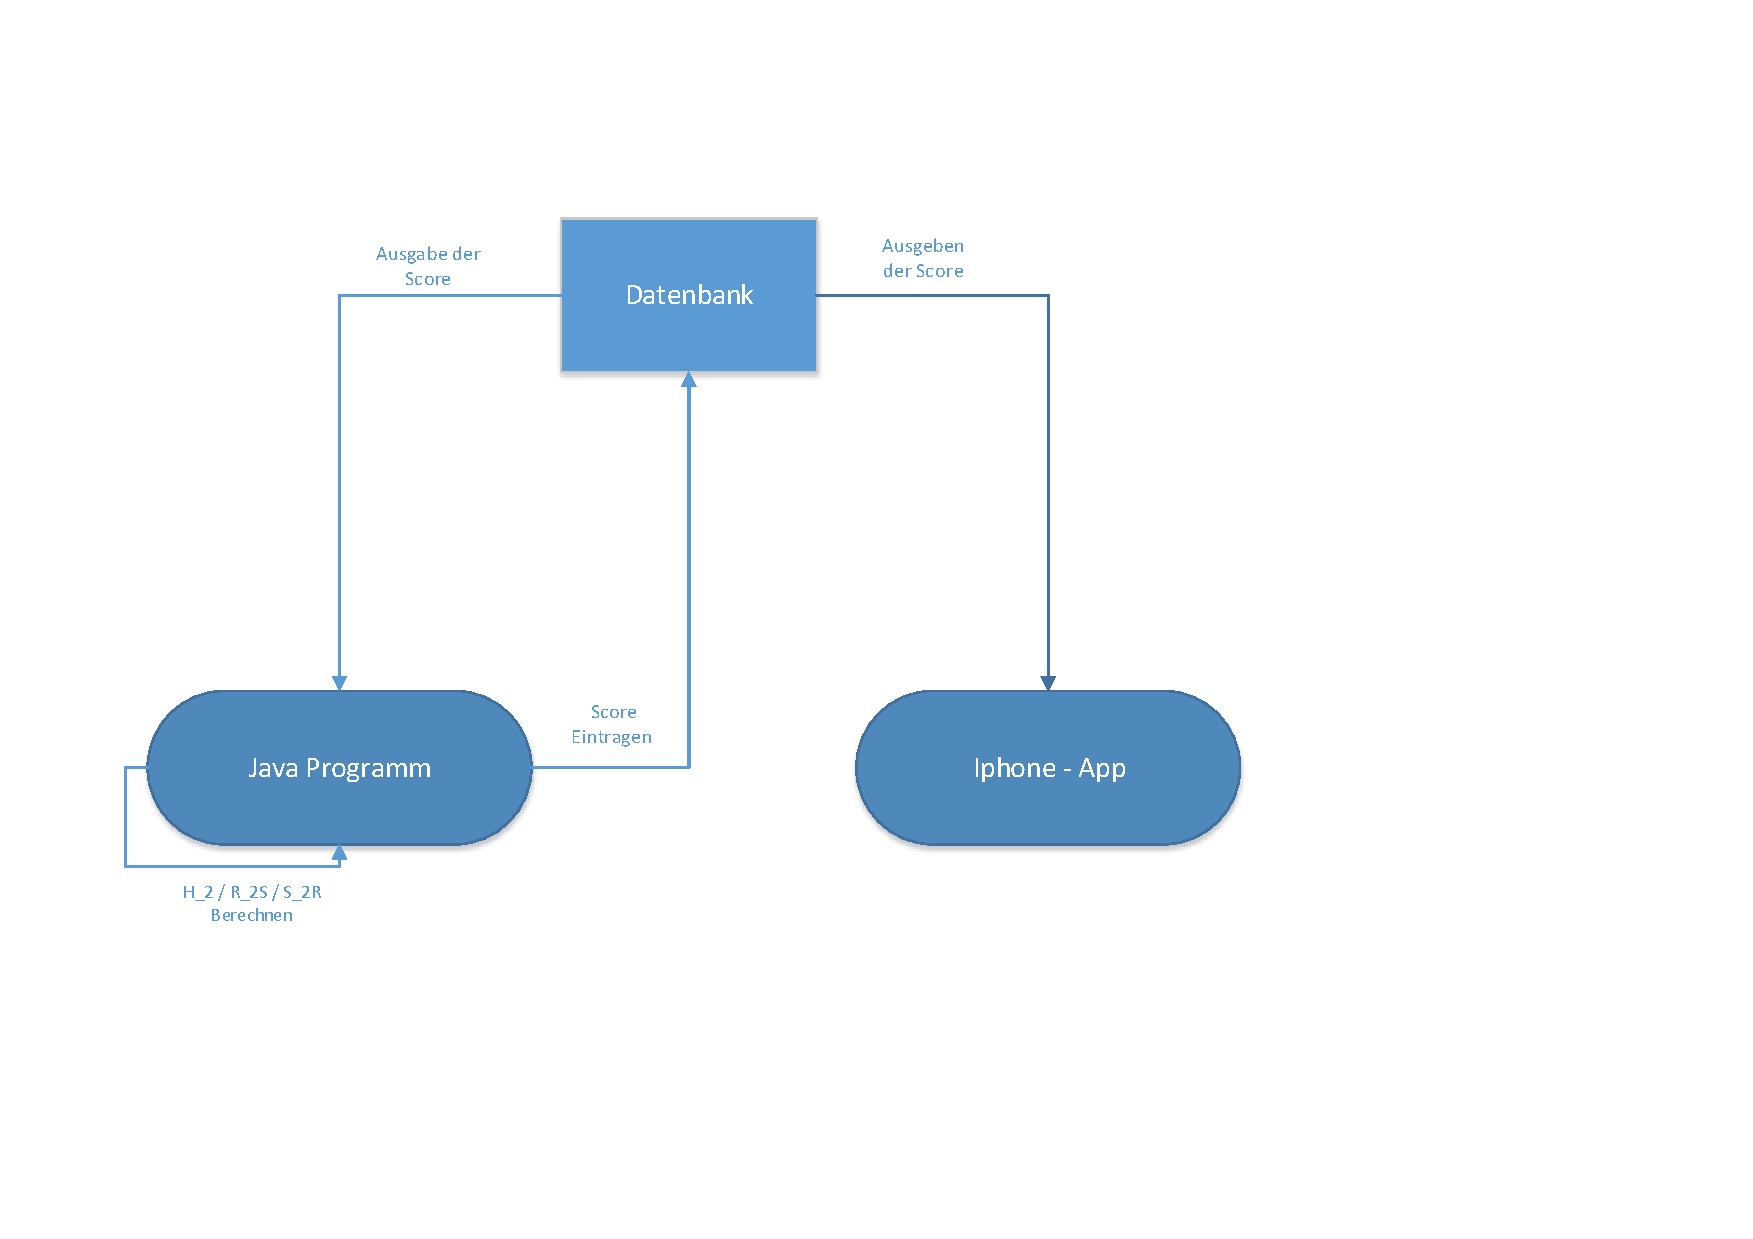
\includegraphics[width=0.7\textwidth]{img/DTD_2_JavaDB.pdf}
		\caption{Datenfluss Java-Datenbank}
	\end{figure}
	\begin{figure}
		\centering
		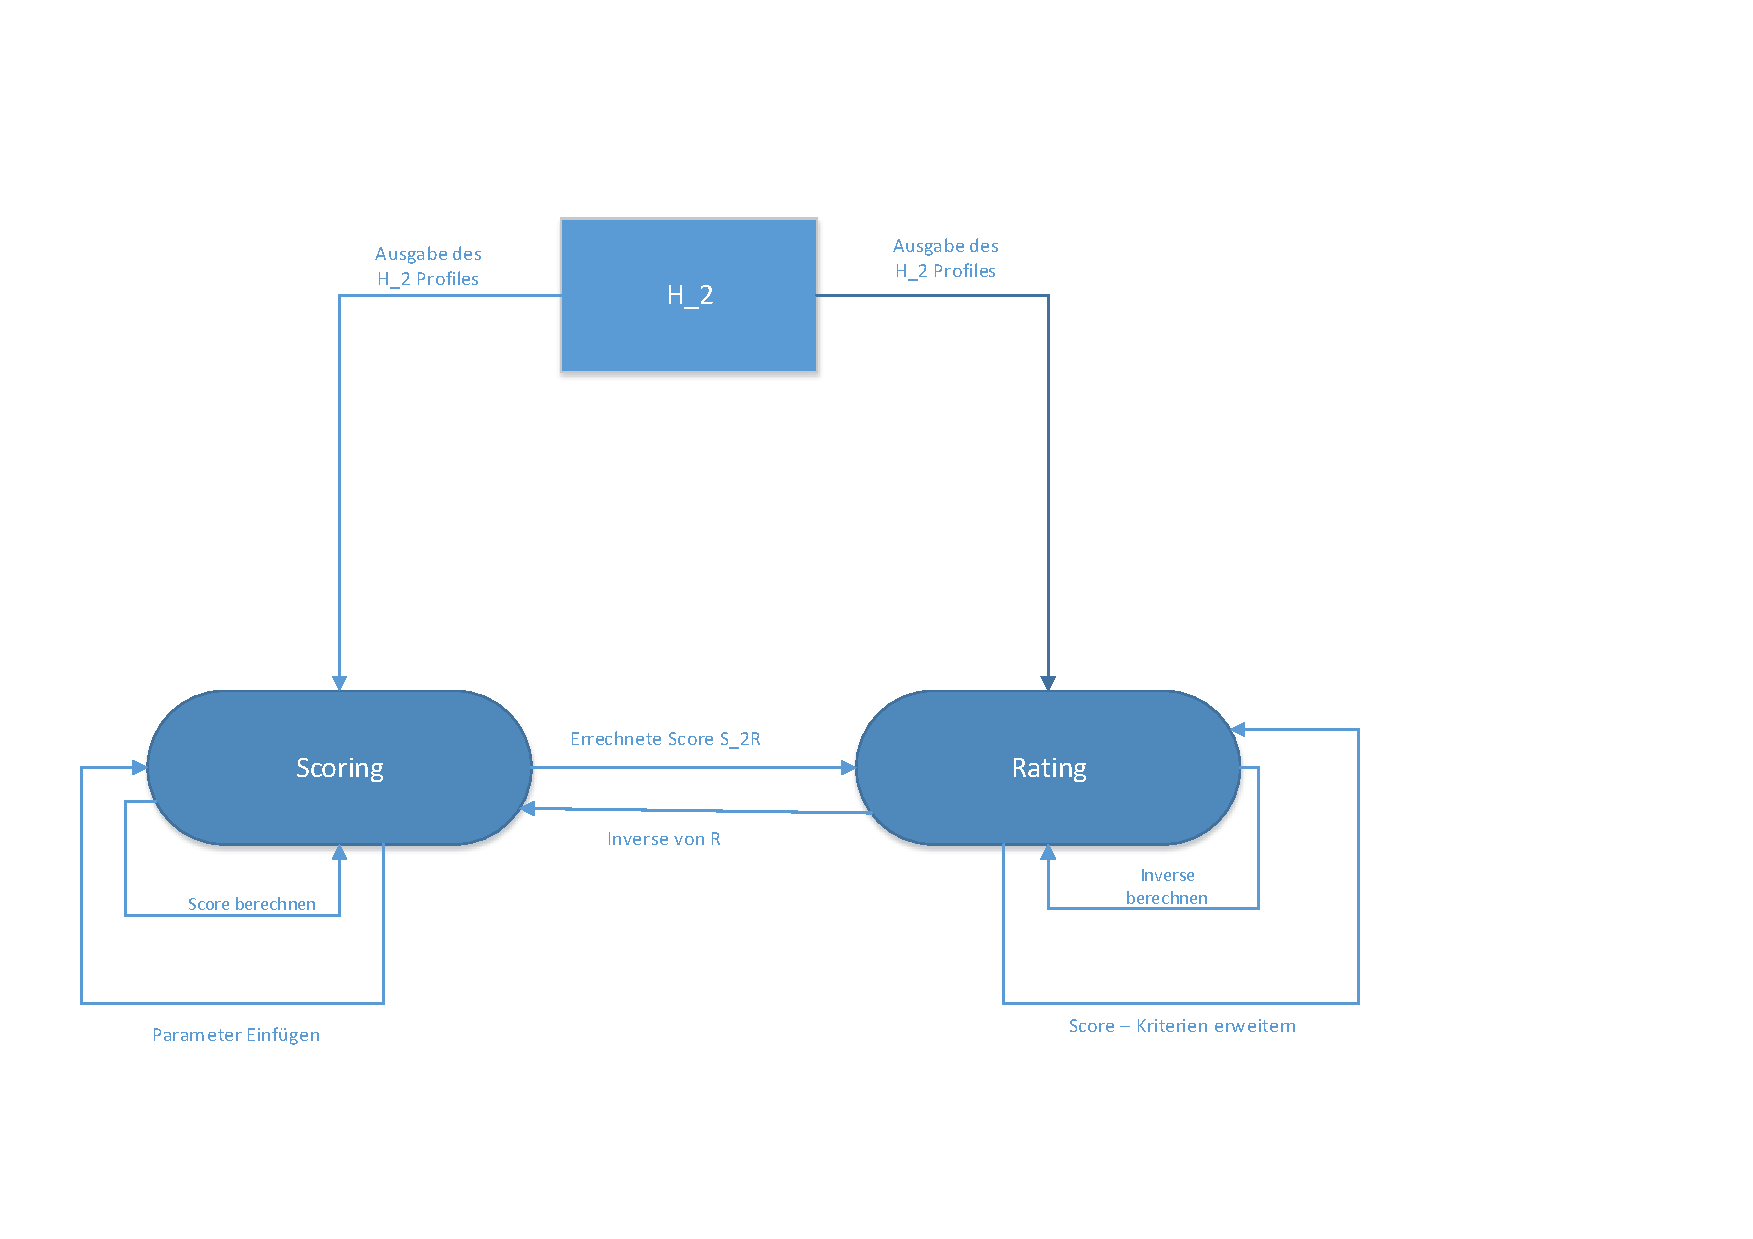
\includegraphics[width=0.7\textwidth]{img/DTD_3_H2SR.pdf}
		\caption{Datenfluss Umrechnung S2R, H2, R2S}
	\end{figure}
	
	
	\listoftables
		
\end{document}